\documentclass[11pt,a4paper,USenglish]{article} % change ``USenglish'' to ``norsk'' if applicable

\usepackage{ttk4135LabReport}

\usepackage{babel}
\usepackage{amsmath,amssymb}
\usepackage[latin1]{inputenc}	
\usepackage{graphicx}
\usepackage{epstopdf}
\usepackage[round]{natbib}
\usepackage{tocbibind}
\usepackage{siunitx}
\usepackage{listings, courier, color}
\usepackage{pgfplots}%Funktionen plotten
\pgfplotsset{compat=newest}
\pgfplotsset{ylabsh/.style={every axis y label/.style={at={(0,0.5)}, xshift=#1, rotate=90}}}
\usetikzlibrary{pgfplots.groupplots}
\usepgfplotslibrary{external}
\tikzexternalize[shell escape=-shell-escape]
\tikzsetexternalprefix{pgfplots/}

\usepackage[hidelinks]{hyperref} % Always load last
\usepackage{cleveref} % cleveref goes laster

\studentnumbers{750001, 750002, 750003, and 750004 (Tor Aksel Heirung)}
\groupnumber{4?}
\date{\today}

\begin{document}
	
\renewcommand{\d}{\mathrm{d}}
\renewcommand{\j}{\mathrm{j}}
\newcommand{\e}{\mathrm{e}}
\renewcommand{\vec}[1]{\mathbf{#1}}
\newcommand{\mybr}[1]{\left(#1\right)}
\providecommand{\with}{\,, & \qquad}
\providecommand{\FullStop}{\text{~\@.}}
\providecommand{\Comma}{\text{~,}}

\newcommand{\ProblemTwoPlot}[2]{
	\begin{tikzpicture}
	\begin{groupplot}[
	group style={
		group name=ioverlauf,
		group size=1 by 4,
		%
		%xlabels at=edge bottom,
		ylabels at=edge left,
		x descriptions at=edge bottom,
		horizontal sep=1.25cm,
		vertical sep=0.375cm
	},
	width=0.95\linewidth,
	height=0.28\textheight,
	grid,
	xlabel={$t$ in \si{\second}},
	ylabsh=-3.5em
	]
	\nextgroupplot[ 
	ylabel={$\lambda$} in \si{\degree},legend to name=travel]
	\addplot[color=blue] table[x=t,y expr=\thisrow{lambda}+180] {#1};
	\addlegendentry{measured}
	\addplot[color=red, const plot] table[x=t,y expr=\thisrow{lambda}*180/pi] {#2};
	\addlegendentry{optimal}
	
	\nextgroupplot[ 
	ylabel={$p$} in \si{\degree},legend to name=pitch]
	\addplot[color=blue] table[x=t,y=p] {#1};
	\addlegendentry{measured}
	\addplot[color=red, const plot] table[x=t,y expr=\thisrow{p}*180/pi] {#2};
	\addlegendentry{optimal}
	
	\nextgroupplot[ 
	ylabel={$e$} in \si{\degree},legend to name=elevation]
	\addplot[color=blue] table[x=t,y=e] {#1};
	\addlegendentry{measured}
	
	\nextgroupplot[ 
	ylabel={$u$} in \si{1},legend to name=input]
	\addplot[color=blue] table[x=t,y=u] {#1};
	\addlegendentry{measured}
	\addplot[color=red, const plot] table[x=t,y=u] {#2};
	\addlegendentry{optimal}
	
	\end{groupplot}
	
	\node at (ioverlauf c1r1.east) [anchor=east, xshift=-0.3cm, yshift=0.0cm]
	{\pgfplotslegendfromname{travel}};
	\node at (ioverlauf c1r2.east) [anchor=east, xshift=-0.3cm, yshift=1.5cm]
	{\pgfplotslegendfromname{pitch}};
	\node at (ioverlauf c1r3.east) [anchor=east, xshift=-0.3cm, yshift=0.0cm]
	{\pgfplotslegendfromname{elevation}};
	\node at (ioverlauf c1r4.east) [anchor=east, xshift=-0.3cm, yshift=1.5cm]
	{\pgfplotslegendfromname{input}};
	
	\end{tikzpicture}
}


\newcommand{\ProblemThreePlot}[2]{
	\begin{tikzpicture}
	\begin{groupplot}[
	group style={
		group name=ioverlauf,
		group size=1 by 4,
		%
		%xlabels at=edge bottom,
		ylabels at=edge left,
		x descriptions at=edge bottom,
		horizontal sep=1.25cm,
		vertical sep=0.375cm
	},
	width=0.95\linewidth,
	height=0.28\textheight,
	grid,
	xlabel={$t$ in \si{\second}},
	ylabsh=-3.5em
	]
	\nextgroupplot[ 
	ylabel={$\lambda$} in \si{\degree},legend to name=travel]
	\addplot[color=blue] table[x=t,y expr=\thisrow{lambda}+180] {#1};
	\addlegendentry{measured}
	\addplot[color=red, const plot] table[x=t,y expr=\thisrow{lambda}*180/pi] {#2};
	\addlegendentry{optimal}
	
	\nextgroupplot[ 
	ylabel={$p$} in \si{\degree},legend to name=pitch]
	\addplot[color=blue] table[x=t,y=p] {#1};
	\addlegendentry{measured}
	\addplot[color=red, const plot] table[x=t,y expr=\thisrow{p}*180/pi] {#2};
	\addlegendentry{optimal}
	
	\nextgroupplot[ 
	ylabel={$e$} in \si{\degree},legend to name=elevation]
	\addplot[color=blue] table[x=t,y=e] {#1};
	\addlegendentry{measured}
	
	\nextgroupplot[ 
	ylabel={$u$} in \si{1},legend to name=input]
	\addplot[color=blue] table[x=t,y=u] {#1};
	\addlegendentry{measured}
	\addplot[color=green, const plot] table[x=t,y=uopt] {#1};
	\addlegendentry{optimal measured?}
	\addplot[color=red, const plot] table[x=t,y=u] {#2};
	\addlegendentry{optimal}
	
	\end{groupplot}
	
	\node at (ioverlauf c1r1.east) [anchor=east, xshift=-0.3cm, yshift=0.0cm]
	{\pgfplotslegendfromname{travel}};
	\node at (ioverlauf c1r2.east) [anchor=east, xshift=-0.3cm, yshift=1.5cm]
	{\pgfplotslegendfromname{pitch}};
	\node at (ioverlauf c1r3.east) [anchor=east, xshift=-0.3cm, yshift=0.0cm]
	{\pgfplotslegendfromname{elevation}};
	\node at (ioverlauf c1r4.east) [anchor=east, xshift=-0.3cm, yshift=1.3cm]
	{\pgfplotslegendfromname{input}};
	
	\end{tikzpicture}
}

\newcommand{\ProblemFourPlot}[2]{
	\begin{tikzpicture}
	\begin{groupplot}[
	group style={
		group name=ioverlauf,
		group size=1 by 5,
		%
		%xlabels at=edge bottom,
		ylabels at=edge left,
		x descriptions at=edge bottom,
		horizontal sep=1.25cm,
		vertical sep=0.375cm
	},
	width=0.95\linewidth,
	height=0.24\textheight,
	grid,
	xlabel={$t$ in \si{\second}},
	ylabsh=-3.5em
	]
	\nextgroupplot[ 
	ylabel={$\lambda$} in \si{\degree},legend to name=travel]
	\addplot[color=blue] table[x=t,y expr=\thisrow{lambda}+180] {#1};
	\addlegendentry{measured}
	\addplot[color=red, const plot] table[x=t,y expr=\thisrow{lambda}*180/pi] {#2};
	\addlegendentry{optimal}
	
	\nextgroupplot[ 
	ylabel={$p$} in \si{\degree},legend to name=pitch]
	\addplot[color=blue] table[x=t,y=p] {#1};
	\addlegendentry{measured}
	\addplot[color=red, const plot] table[x=t,y expr=\thisrow{p}*180/pi] {#2};
	\addlegendentry{optimal}
	
	\nextgroupplot[ 
	ylabel={$e$} in \si{\degree},legend to name=elevation]
	\addplot[color=blue] table[x=t,y=e] {#1};
	\addlegendentry{measured}
	\addplot[color=red, const plot] table[x=t,y expr=\thisrow{e}*180/pi] {#2};
	\addlegendentry{optimal}
	
	\nextgroupplot[ 
	ylabel={$u_1$} in \si{1},legend to name=input1]
	\addplot[color=blue] table[x=t,y=u1] {#1};
	\addlegendentry{measured}
	\addplot[color=green, const plot] table[x=t,y=u1opt] {#1};
	\addlegendentry{optimal measured?}
	\addplot[color=red, const plot] table[x=t,y=u1] {#2};
	\addlegendentry{optimal}
	
	\nextgroupplot[ 
	ylabel={$u_2$} in \si{1},legend to name=input2]
	\addplot[color=blue] table[x=t,y=u2] {#1};
	\addlegendentry{measured}
	\addplot[color=green, const plot] table[x=t,y=u2opt] {#1};
	\addlegendentry{optimal measured?}
	\addplot[color=red, const plot] table[x=t,y=u2] {#2};
	\addlegendentry{optimal}
	
	\end{groupplot}
	
	\node at (ioverlauf c1r1.east) [anchor=east, xshift=-0.3cm, yshift=0.0cm]
	{\pgfplotslegendfromname{travel}};
	\node at (ioverlauf c1r2.east) [anchor=east, xshift=-0.3cm, yshift=-1.0cm]
	{\pgfplotslegendfromname{pitch}};
	\node at (ioverlauf c1r3.east) [anchor=east, xshift=-0.3cm, yshift=-1.0cm]
	{\pgfplotslegendfromname{elevation}};
	\node at (ioverlauf c1r4.east) [anchor=east, xshift=-0.3cm, yshift=1.3cm]
	{\pgfplotslegendfromname{input1}};
	\node at (ioverlauf c1r5.east) [anchor=east, xshift=-0.3cm, yshift=0.8cm]
	{\pgfplotslegendfromname{input2}};
	
	\end{tikzpicture}
}

\makelabreportfrontpage

\begin{abstract}\addcontentsline{toc}{section}{Abstract}
This document outlines a few important aspects of the lab report. It contains some advice on both content and layout. The Latex source for this document is also published, and you can use it as a template of sorts for your own report.

When you write your own report, this section (the abstract) should contain a \emph{very} short summary of what the lab is about and what you have done.
\end{abstract}

\tableofcontents

\section{Introduction}
In this lab we are going to use the techniques and theory taught in the course of optimization theory and control. To control a small helicopter model. We will be doing this by computing the optimal trajectory of the helicopter and give a corresponding input for this trajectory.

To compute this we need to derive a non-linear model for the dynamics of the system. Then linearize the model around an equilibrium. (add more context)

We will try out a few different setup to measure the performance of the optimal control computed. One where we use the optimal input directly without any feedback. Also we will try to compensate for the inaccuracy of the model by using a feedback controller. In this lab we will be using an linear-quadratic regulator to control the feedback loop.

OLD
Your introduction should contain an overview of the work you were assigned, as well as a few sentences putting the work into a larger perspective. You should also give a quick description of how the report is organized (as is done below).

You should of course put most of the work into doing good work in the lab and then presenting it in the report. When presenting your work in the report, both content and presentation/layout matters. Since your only way of communicating your good effort in the lab is through writing about it here, the way you write about it is essential. This means that even if you have the very best controller but describe it poorly, you will probably not be rewarded for the good results. A plot showing perfect control is worth very little if it is not accompanied by a clear description of what it represents.

Layout is naturally less important than content, but it still matters. You can think of report writing like selling an apartment; when you present your apartment for potential buyers you will of course clean the apartment and make it good looking. How clean the apartment is does of course not determine its value, but it is still important since it influences the subjective value your buyers will put on the apartment. 

\subsection{Software}
You are of course free to use whatever software you want for report writing. You can also submit a handwritten report, although this is probably not a great idea if your handwriting can be hard to read. 

You can also use Word or a similar word processor. However, it is next to impossible to achieve decent layout with Word. The support for vector graphics (discussed later) is extremely poor, and text tends to look pretty bad (bad support for kerning and ligatures). Furthermore, math is both time consuming and difficult to input, and tends to look very ugly. In general, a report written in Word looks like a draft.

It is strongly recommended to use Latex. Unless you tweak the layout too much, your report will almost certainly look very good. Although it can take a bit of effort to get started, it is also much quicker to use than Word and similar programs. The support for math and vector graphics is also great.

If you are new to Latex, you can have a look at the source for this document to get started. You can also look at the presentation by \citet{Berland2010} (in Norwegian) or consult \citet{Oetiker2011}. Another good reason to learn Latex is that you probably don't want to write your master's thesis in something like Word, doing so would likely be very frustrating. Being reasonably fluent in Latex before you get that far will make your thesis work much smoother.

Some of you are probably fluent in Latex and might plan to write the report using it. Please resist the temptation (if any) to change the fonts, make super fancy headers (they are not necessary for a report like this), change the margins, change the paragraph indentation and/or spacing, and similar things.

A great tool for collaborating on Latex documents is ShareLaTeX at \url{https://www.sharelatex.com/}; if you use this you won't have to install anything on your computer. Texmaker at \url{http://www.xm1math.net/texmaker/} is a good cross-platform editor. Some people like Lyx, which is a Latex editor that behaves a little bit like Word.

\subsection{Other Comments}
If you have problems with Latex, the solution is usually just a few Google searches away.

You can write the report in Norwegian or English. Writing in English is encouraged and is great practice, but entirely optional. \emph{Do not interpret any of the advice or suggestions here as requirements.}

This report is organized as follows: Section~\ref{sec:prob_descr} contains a few remarks on report writing and some random Latex advice. An example of a table can be foundin Section~\ref{sec:prob1}, along with two remarks on report writing. Section~\ref{sec:prob2} contains some advice on using plots from MATLAB. A few suggestions for making illustrations are given in Section~\ref{sec:prob3}; a matrix equation can also be found here. Section~\ref{sec:prob4} has a few comments on references and floats in Latex. The closing discussion and concluding remarks are in Sections~\ref{sec:discussion} and~\ref{sec:conclusion}, respectively. Appendix~\ref{sec:matlab} contains a MATLAB file while Appendix~\ref{sec:simulink} shows an example Simulink diagram. The Bibliography can be found at the end, on page~\pageref{sec:bibliography}.
%\section{Problem Description}\label{sec:prob_descr}
In this section you should describe the lab setup and discuss the model. If you want, you can copy the source code for the model equations:
\begin{gather}
	\ddot{e} + K_{3} K_{ed} \dot{e} + K_{3} K_{ep} e = K_{3} K_{ep} e_{c} \label{eq:model_elev} \\
	\ddot{p} + K_{1} K_{pd} \dot{p} + K_{1} K_{pp} p = K_{1} K_{pp} p_{c} \label{eq:model_pitch} \\
	\dot{\lambda} = r \label{eq:model_lambda} \\
	\dot{r} = -K_{2} p \label{eq:model_r} 
\end{gather}
Since these equations belong together, it's a good idea to number them like this:
\begin{subequations}
\label{eq:model}
\begin{gather}
	\ddot{e} + K_{3} K_{ed} \dot{e} + K_{3} K_{ep} e = K_{3} K_{ep} e_{c} \label{eq:model_se_elev} \\
	\ddot{p} + K_{1} K_{pd} \dot{p} + K_{1} K_{pp} p = K_{1} K_{pp} p_{c} \label{eq:model_se_pitch} \\
	\dot{\lambda} = r \label{eq:model_se_lambda} \\
	\dot{r} = -K_{2} p \label{eq:model_se_r} 
\end{gather}
\end{subequations}
You can then both reference individual equations (``the elevation equation \eqref{eq:model_se_elev}'') or reference the entire model (``the linear model \eqref{eq:model}''). Regardless of your choice of software, never hard-code a reference, always use dynamic references. 

You could also align the equations like this:
\begin{subequations}
\label{eq:model_al}
\begin{align}
	\ddot{e} + K_{3} K_{ed} \dot{e} + K_{3} K_{ep} e &= K_{3} K_{ep} e_{c} \label{eq:model_se_al_elev} \\
	\ddot{p} + K_{1} K_{pd} \dot{p} + K_{1} K_{pp} p &= K_{1} K_{pp} p_{c} \label{eq:model_se_al_pitch} \\
	\dot{\lambda} &= r \label{eq:model_se_al_lambda} \\
	\dot{r} &= -K_{2} p \label{eq:model_se_al_r} 
\end{align}
\end{subequations}
You can consult \citet{Downes2002} for more about writing math.

If you decide to include a figure, that's great. You can in general copy figures from the textbook, the assignement text, or other places. However: ALWAYS CITE THE SOURCE.
\section{Repetition/Introduction to Simulink/QuaRC}\label{sec:prob1}
This section should not be very long.

If you want, you can use the source for Table~\ref{tab:parameters} to see how a (floating) table is made. 

Variables and symbols are always in italics, while units are not.

\begin{table}[tbp]
	\centering
	\caption{Parameters and values.}
	\begin{tabular}{llls}
		\hline
		Symbol & Parameter & Value & Unit \\
		\hline
		$l_a$ & Distance from elevation axis to helicopter body & $0.63$ & \meter \\
		$l_h$ & Distance from pitch axis to motor & $0.18$ & \meter \\
		$K_f$ & Force constant motor & $0.25$ & \newton\per\volt \\
		$J_e$ & Moment of inertia for elevation & $0.83$ & \kilogram\square\meter \\
		$J_t$ & Moment of inertia for travel & $0.83$ & \kilogram\square\meter \\
		$J_p$ & Moment of inertia for pitch & $0.034$ & \kilogram\square\meter \\
		$m_h$ & Mass of helicopter & $1.05$ & \kilogram \\
		$m_w$ & Balance weight & $1.87$ & \kilogram \\
		$m_g$ & Effective mass of the helicopter & $0.05$ & \kilogram \\
		$K_p$ & Force to lift the helicopter from the ground & $0.49$ & \newton \\
		\hline
	\end{tabular}
	\label{tab:parameters}
\end{table}

\section{Optimal Control of Pitch/Travel without Feedback}\label{sec:prob2}

\subsection{State space form}\label{sec:prob21}
For Problem 2 an optimal control sequence had to be calculated disregarding the elevation \emph{e} and relinquishing feedback. The states were given by the problem description with $\mathbf{x}= \begin{bmatrix} \lambda & r & p & \dot p \end{bmatrix}^\top$ and the only input was given by $u = p_c$. Therefore the model can be written in time state space form in the following way: 
\begin{equation} \label{statespace2}
	\underbrace{\begin{bmatrix}
		\dot \lambda \\
		\dot r \\
		\dot p \\
		\ddot p
	\end{bmatrix}}_\text{$\mathbf{\dot x}$}
	=
	\underbrace{\begin{bmatrix}	
				0 & 1 & 0 & 0 \\
				0 & 0 & -K_2	& 0 \\
				0 & 0 & 0 & 1 \\
				0 & 0 & -K_1K_{pp} & -K_1K_{pd}
	\end{bmatrix}}_\text{$\mathbf{A_c}$}
	\underbrace{\begin{bmatrix}
		\lambda \\
		r \\
		p \\
		\dot p
	\end{bmatrix}}_\text{$\mathbf{x}$}
	+
	\underbrace{\begin {bmatrix}	
				0 \\
				0 \\
				0 \\
				K_1K_{pp}			
	\end{bmatrix}}_\text{$\mathbf{B_c}$}
	\underbrace{
		\vphantom { 
			\begin {bmatrix}	
				0 \\
				0 \\
				0 \\
				K_1K_{pp}			
			\end{bmatrix}
		}
		p_c
	}_\text{u}
\end{equation}

\subsection{Discussion of the model}\label{sec:prob22}
The control hierarchy of the model is displayed in following figure:
\begin{figure}[h]
	\centering
	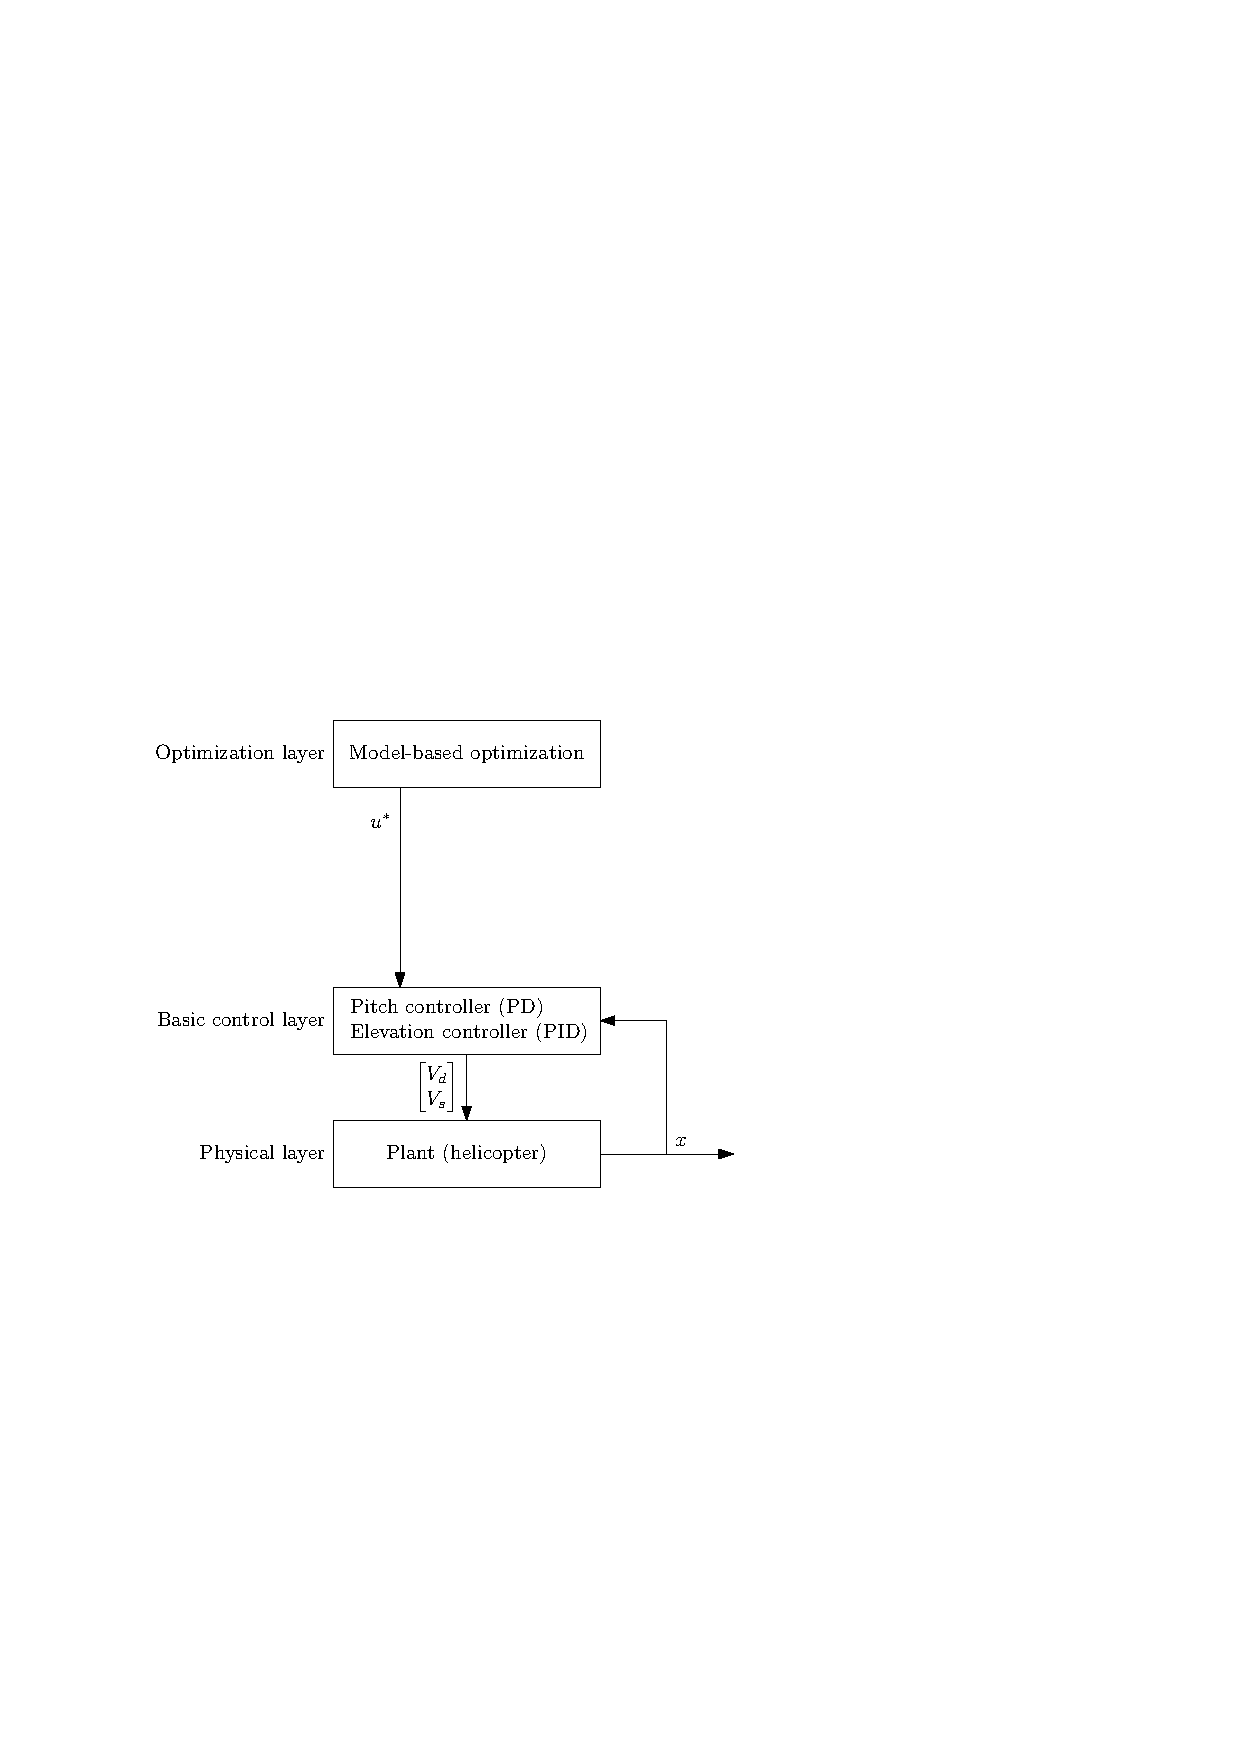
\includegraphics[width=1.0\textwidth]{figures/layers_openloop.pdf}
	\caption[Control hierarchy as used in Problem 2]{Control hierarchy\footnotemark as used in Problem 2}
	\label{fig:layers_openloop}
\end{figure}
\footnotetext {as depicted in the problem description}
\newline
Since the model as presented above also contains the pitch and elevation setpoints as inputs it does not only depict the phyiscal behaviour of the helicopter. Instead also the inner control loops of pitch and elevation are modeled.
\subsection{Discretisation}\label{sec:prob23}
In order to use the time state space form to calculate the optimal trajectory from the optimal control sequence it had to be discretised in time. For the discretisation the forward Euler method was used:
\begin{equation}
	\mathbf{x_{k+1}}= \mathbf{x_k}+ \Delta t \mathbf{\dot x_k}
\end{equation}
using the time state space form (\ref{statespace2})
\begin{align}
	\mathbf{x_{k+1}}&=\mathbf{x_k+ (A_cx_k+B_c}u_k) \Delta t \nonumber \\ 
			&=(\mathbf{I} + \Delta t\mathbf{ A_c})\mathbf{x_k}+\Delta t \mathbf{B_c}u_k \nonumber \\
			&=\mathbf{Ax_k+B}u_k
\end{align}
\begin{equation}
	\mathbf{A} =
	\begin{bmatrix}
				1 & \Delta t & 0 & 0 \\
				0 & 1 & -K_2\Delta t& 0 \\
				0 & 0 & 1 & \Delta t \\
				0 & 0 & -K_1K_{pp}\Delta t & 1-K_1K_{pd}\Delta t
	\end{bmatrix}, \quad
	\mathbf{B} =
	\begin{bmatrix}	
				0 \\
				0 \\
				0 \\
				K_1K_{pp}\Delta t			
	\end{bmatrix}
\end{equation}
For the discretisation a time step $\Delta t = 0.25 \mathrm{s}$ was used.

\subsection{Optimal trajectory}\label{sec:prob24}
For the starting point $\mathbf{x_0} = \begin{bmatrix} \lambda_0&0&0&0\end{bmatrix}^\top$ and the terminal point $\mathbf{x_f}=  \begin{bmatrix} \lambda_f&0&0&0\end{bmatrix}^\top$ the optimal trajectory had to be calculated. $\lambda_0$ was set to $\pi$ and $\lambda_f$ was set to $0$.So the helicopter should make a curve of 180\textdegree and then remain at his position. In order to find the optimal trajectory the following cost function was minimised with different weightings $q$ for the pitch input $p_{ci}$:
\begin{equation}
\phi = \displaystyle\sum_{i=1}^{N} (\lambda_i-\lambda_f)^2+qp_{ci}^2, \quad q \geq 0
\end{equation}
Additionally the following constraint on the input value was implemented:
\begin{equation}
	|p_k|\leq \frac {30\pi} {180}, \quad k \in \{1, \dots,N\}
\end{equation}
The constraint prevents the helicopter from flying rather extreme manoeuvres where the pitch angle exceeds 30\textdegree and thus contributes to the overall safety of the equipment and the laboratory staff. Since the cost function is quadratic in both variables, the pitch input and the deviation of the position from the terminal point, it can be solved by quadratic programming algorithms. Though the helicopters position will always be compared to the terminal point. This may result in fast helicopter movement and aggressive steering, which can be hard to handle due to the helicopter's momentum. High pitch angles may also exceed the area in which the system equation are sufficiently accurate since they rely on small angle approximations. Also aggressive inputs on the pitch control may cause the pitch angle to exceed the constraints due to the momentum of the helicopter.

The MATLAB code can be seen in \cref{sec:problem2_m} and the Simulink diagram can be seen in \cref{fig:problem2_simulink}.

\subsection{Results of the optimization}\label{sec:prob25}
To solve the optimization problem the $\mathrm{MATLAB}$ function \texttt{quadprog} was used. Values of 0.1, 1, and 10 were chosen for the weighting factor $q$. 5 seconds of zeroes were added before and after the control sequence in order to give the helicopter some time to stabilise. The results were exported from $\mathrm{MATLAB}$ and are depicted in the Figures (\ref{fig:problem2plots_q_1.0}),  (\ref{fig:problem2plots_q_0.1}) and  (\ref{fig:problem2plots_q_10}).
\begin{figure}[h]
	\centering
	\ProblemTwoPlot{../MATLAB/Export/problem2plots_q_1.0.csv}{../MATLAB/Export/problem2plots_q_1.0_opt.csv}
	\caption{Results for $R=1.0$}
	\label{fig:problem2plots_q_1.0}
\end{figure}

\begin{figure}[h]
	\centering
	\ProblemTwoPlot{../MATLAB/Export/problem2plots_q_0.1.csv}{../MATLAB/Export/problem2plots_q_0.1_opt.csv}
	\caption{Results for $R=0.1$}
	\label{fig:problem2plots_q_0.1}
\end{figure}

\begin{figure}[h]
	\centering
	\ProblemTwoPlot{../MATLAB/Export/problem2plots_q_10.csv}{../MATLAB/Export/problem2plots_q_10_opt.csv}
	\caption{Results for $R=10$}
	\label{fig:problem2plots_q_10}
\end{figure}

As expected a lower value for $q$ allows much stronger inputs than higher values. This is logical since a higher value for $q$ emphasizes the influence of the inputs in the cost function. Therefore the higher $q$ is the less inputs are given in order to keep the value of the cost function low. Still, regardless of the value of $q$ the helicopter does not remain at his terminal point but continues moving as we can see in the plot of $\lambda$. This behaviour can be ascribed to the missing feedback. The helicopter does only follow the control sequence that has been calculated in advance and does not compare the setpoints with his current state. 




\section{Optimal Control of Pitch/Travel with Feedback (LQ)}\label{sec:prob3}
You are as mentioned welcome to use the figures from the assignment text if you want to (cite the source!). You can also draw your own (cite the source if it is heavily based on someone else's.). Figure~\ref{fig:layers_openloop} was created quickly with Ipe. Inkscape is a good alternative for more advanced illustrations. Some people prefer the Latex package TikZ (\url{http://texample.net/tikz/examples/}), but this takes a little effort to learn.

\begin{figure}[tp]
	\centering
		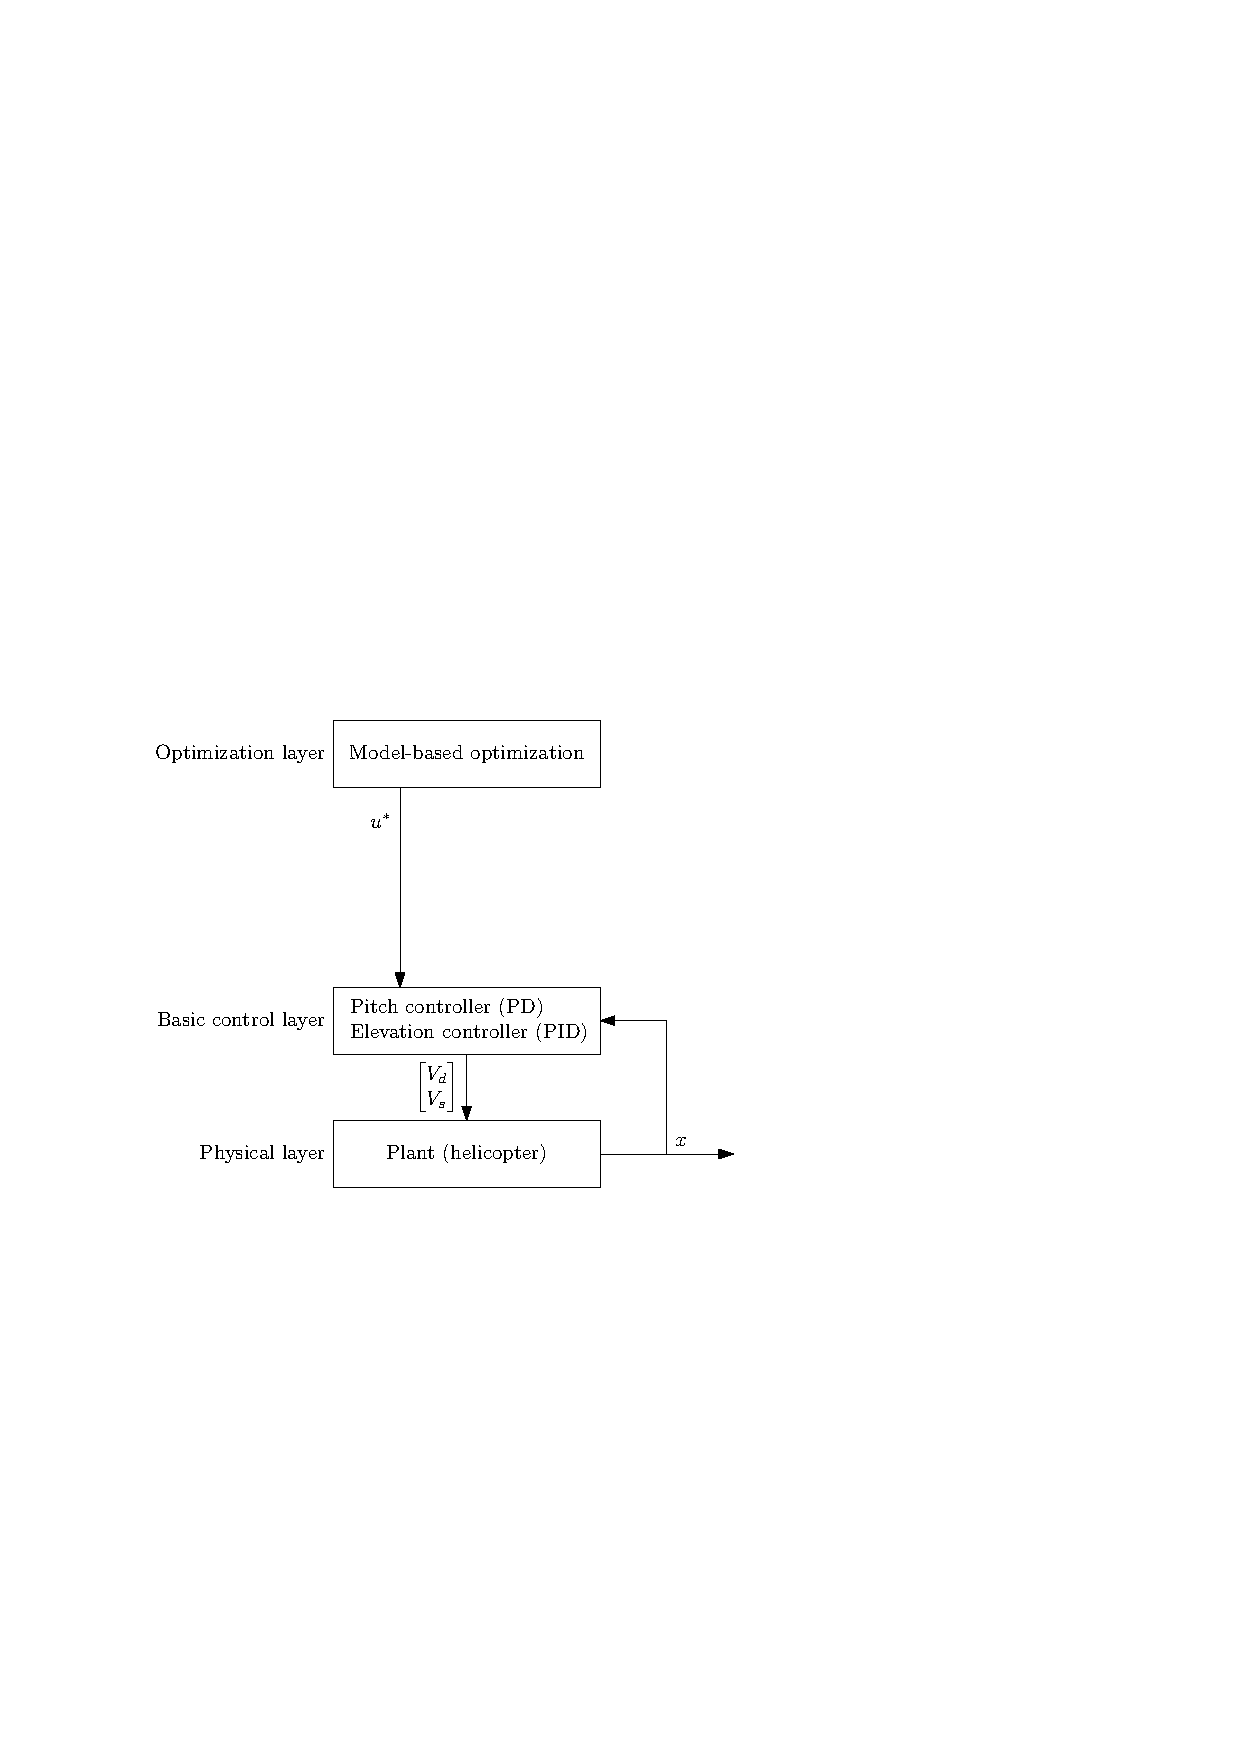
\includegraphics[width=1.00\textwidth]{figures/layers_openloop.pdf}
	\caption{A figure created with Ipe.}
	\label{fig:layers_openloop}
\end{figure}

Here is a matrix equation you can use as a template:
\begin{equation}
\begin{bmatrix}
 1 &  0 &  0 & 0 & -b &  0 &  0 &  0 \\
-a &  1 &  0 & 0 &  0 & -b &  0 &  0 \\
 0 & -a &  1 & 0 &  0 &  0 & -b &  0 \\
 0 &  0 & -a & 1 &  0 &  0 &  0 & -b                                
\end{bmatrix}
\begin{bmatrix} x_1 \\ x_2 \\ x_3 \\ x_4 \\ u_0 \\ u_1 \\ u_2 \\ u_3 \end{bmatrix}
=
\begin{bmatrix}
ax_0 \\ 0 \\ 0 \\ 0      
\end{bmatrix}
\end{equation}




\begin{figure}[htbp]
	\centering
	\ProblemThreePlot{../MATLAB/Export/problem3plot_1010_1.csv}{../MATLAB/Export/problem2plots_q_10_opt.csv}
	\caption{problem3plot\_1010\_1}
	\label{fig:problem3plot_1010_1}%
\end{figure}

\begin{figure}[htbp]
	\centering
	\ProblemThreePlot{../MATLAB/Export/problem3plot_1050_1.csv}{../MATLAB/Export/problem2plots_q_10_opt.csv}
	\caption{problem3plot\_1050\_1}
	\label{fig:problem3plot_1050_1}%
\end{figure}

\begin{figure}[htbp]
	\centering
	\ProblemThreePlot{../MATLAB/Export/problem3plot_5010_1.csv}{../MATLAB/Export/problem2plots_q_10_opt.csv}
	\caption{problem3plot\_5010\_1}
	\label{fig:problem3plot_5010_1}%
\end{figure}

\begin{figure}[htbp]
	\centering
	\ProblemThreePlot{../MATLAB/Export/problem3plot_10150_0.5.csv}{../MATLAB/Export/problem2plots_q_10_opt.csv}
	\caption{problem3plot\_10150\_0.5}
	\label{fig:problem3plot_10150_0.5}%
\end{figure}


\begin{figure}[htbp]
	\centering
	\ProblemThreePlot{../MATLAB/Export/problem3_LQR[1,0,10,0].csv}{../MATLAB/Export/problem2plots_q_10_opt.csv}
	\caption{problem3\_LQR[1,0,10,0], R = 0.5}
	\label{fig:problem3_LQR[1,0,10,0]}%
\end{figure}

\begin{figure}[htbp]
	\centering
	\ProblemThreePlot{../MATLAB/Export/problem3_LQR[1,0,10,10].csv}{../MATLAB/Export/problem2plots_q_10_opt.csv}
	\caption{problem3\_LQR[1,0,10,10], R = 0.5}
	\label{fig:problem3_LQR[1,0,10,10]}%
\end{figure}

\begin{figure}[htbp]
	\centering
	\ProblemThreePlot{../MATLAB/Export/problem3_LQR[5,0,0,5].csv}{../MATLAB/Export/problem2plots_q_10_opt.csv}
	\caption{problem3\_LQR[5,0,0,5], R = 0.5}
	\label{fig:problem3_LQR[5,0,0,5]}%
\end{figure}

\begin{figure}[htbp]
	\centering
	\ProblemThreePlot{../MATLAB/Export/problem3_LQR[10,1,5,0].csv}{../MATLAB/Export/problem2plots_q_10_opt.csv}
	\caption{problem3\_LQR[10,1,5,0], R = 0.5}
	\label{fig:problem3_LQR[10,1,5,0]}%
\end{figure}
\section{Optimal Control of Pitch/Travel and Elevation with and without Feedback}\label{sec:prob4}
In this part of the excersice a constraint on the elevation is added. Therefore the equation describing the dynamics of the elevation $e$ from \eqref{} must be added to the state space representation of the model of the helicopter
\begin{subequations}
	\begin{equation}
	\frac{\d\vec{x}}{\d t}=\vec{A}_c\vec{x}+\vec{B}_c\vec{u}
	\end{equation}
	with
	\begin{align}
	\vec{A}&=\begin{bmatrix}
    0 & 1 & 0 & 0 & 0 & 0\\ 
	0 & 0 & -K_2 & 0 & 0 & 0\\ 
	0 & 0 & 0 & 1 & 0 & 0\\ 
	0 & 0 & -K_1 K_{pp} & -K_1*K_{pd} & 0 & 0 \\
	0 & 0 & 0 & 0 & 0 & 1\\
	0 & 0 & 0 & 0 & -K_3*K_{ep} & -K_3*K_{ed}
	\end{bmatrix}\\
	\vec{B}&=\begin{bmatrix}
	0 & 0\\ 
	0 & 0\\ 
	0 & 0\\ 
	K_1 K_{pp} & 0\\ 
	0 & 0\\ 
	0 & K_3 K_{ep}
	\end{bmatrix}\\
	\vec{x}&=\begin{bmatrix}
	\lambda &
	r&
	p&
	\dot{p}&
	e&
	\dot{e}
	\end{bmatrix}^T\\
	\vec{u}&=\begin{bmatrix}
	p_c & e_c
	\end{bmatrix}^T
	\FullStop
	\end{align}
\end{subequations}
The new input $e_c$ is the stepoint of the elevation. The continuous model is then converted to a time discrete model 
\begin{equation}
\vec{x}_{t+1}=\vec{A}\vec{x}_t+\vec{B}\vec{u}
\end{equation}with the forward Euler method
\begin{subequations}
	\begin{align}
	\vec{A}&=\vec{I}_{6\times6}+\vec{A}_c \Delta t\\
	\vec{B}&=\vec{B}_c\Delta t
	\end{align}
	\label{eq:problem4_disc_model}%
\end{subequations}
with $\Delta t$ being the sampling time. 

The cost function 
\begin{equation}
\phi=\sum_{i=1}^{N}\mybr{\lambda_i-\lambda_f}^2+q_1p_{ci}^2+q_2e_{ci}^2
\end{equation}
is used as a minimization criteria, with the final value for the travel $\lambda_f=0$ and $q_1=1$ and $q_2=2$. The values for $q_1$ and $q_2$ are chosen this way to reduce the oscillations in the opimal trajectory of $p$ and $\dot{p}$ which occur if $q_1=q_2=1$ is used.

The initial value $\vec{x}_0=\begin{bmatrix}\pi & 0 & 0 & 0 & 0 & 0\end{bmatrix}^T$ is used to ensure a travel distance of $\pi$.


As in \cref{sec:prob2} a constraint of $\pm\SI{30}{\degree}$ is used for the pitch $p$ and the setpoint of the pitch $p_c$. Input constraints of $\pm\SI{60}{\degree}$ for $e_c$ are added to avoid a collision between the helicopter and the table on which the helicopter is mounted. Since \eqref{eq:problem4_disc_model} needs to be valid at each time step the equaions are added as equality constraints
\begin{subequations}
	\begin{align}
	\vec{A}_{eq}&=\begin{bmatrix}
	\vec{I} & \vec{0} & \cdots & \cdots & \vec{0} & -\vec{B} & \vec{0} & \cdots &\cdots & \vec{0}\\
	-\vec{A} & \vec{I} & \ddots & & \vdots & \vec{0} & \ddots & \ddots &  & \vdots\\
	\vec{0} & \ddots & \ddots & \ddots & \vdots & \vdots & \ddots & \ddots & \ddots &\vdots \\
	\vdots & \ddots & \ddots & \ddots & \vec{0} & \vdots &  & \ddots & \ddots &\vec{0} \\
	\vec{0} & \cdots & \vec{0} & -\vec{A} & \vec{I} & \vec{0} & \cdots & \cdots & \vec{0} &-\vec{B}\\
	\vec{0} & \cdots & \cdots & \cdots & \vec{I} & \vec{0} & \cdots & \cdots & \cdots & \vec{0}\\
	\end{bmatrix}\\
	\vec{B}_{eq}&=\begin{bmatrix}
	\vec{A}\vec{x}_0\\
	\vec{0}\\
	\vdots\\
	\vec{0}\\
	\vec{x}_f
	\end{bmatrix}\Comma
	\end{align}
\end{subequations}
with $\vec{x}_f=\begin{bmatrix} 0 & 0 & 0 & 0 & 0 & 0\end{bmatrix}^T$ being the final state at $t=N$. A nonlinear constraint 
\begin{equation}
c\mybr{\vec{x}_k}=\alpha \exp\mybr{-\beta\mybr{\lambda_k-\lambda_t}^2}-e_k\leq0 \quad \forall k\in\{1,\ldots,N\}
\label{eq:problem4_nonlinear_constraint}
\end{equation}
with $\alpha=0.2$, $\beta=20$ and $\lambda_t=\frac{2\pi}{3}$, is added. Since \eqref{eq:problem4_nonlinear_constraint} is nonlinear the optimization problem is nonlinear and therefore a nonlinear solver is used. The MATLAB command \verb|fmincon| with three different algorithms is used. The SQP algorithm converges to a solution where the tarjectory of the travel $\lambda$ consists of a single step from $\pi$ to 0, which is unphysical and therefore cannot be used as a reference trajoctory for the helicopter. The active-set method converges to a solution where the input $u_1$ is \SI{83}{\percent} of the time at saturation limit. Although this is only the open loop trajectory it means that when the loop is closed using the LQR the input is still at the saturation limit (assuming that the model is perfect and that there are no disturbances) which means that the control loop is actually open. Because of that the interior-point method is used which results in an trajectory where the input is only \SI{8}{\percent} of the time at the saturation limit. The computation time for calculating the trajectory are \SI{0.33}{\second} for the SQP method, \SI{8.06}{\second} for the active-set method and \SI{53.51}{\second} for the interior-point method, but this is of little concern since the optimization problem doesn't need to be solved online.

The code for calculating the optimal trajectory is shown in \cref{sec:problem4_m}, the nonlinear constraint function can be seen in \cref{sec:constr4_m} and the calculation of the LQR gain matrix is done in \cref{sec:problem4_lqr_m}. The simulink diagram is shown in \cref{fig:problem4_simulink} and \cref{fig:problem4_lqr_simulink}.

The time curve of the helicopter without feedback can be seen in \cref{fig:problem4plots_without_feedback}. As in \cref{sec:prob2} the trajectory of the pitch $p$ is followed, which is due to the pitch control loop which helps to counteract for modeling errors and that a linear model of the nonlinear system is used. The same applies for the elevation control loop which had a reference point of zero in the last two sections and has a trajectory unequal to zero due to the nonlinear constraint \eqref{eq:problem4_nonlinear_constraint} in this section. The reference trajectory of the travel $\lambda$ is not followed satisfactorily. This is the case because the travel $\lambda$ is constrolled in open loop and due to modeling errors the input is not calculated correctly which causes the severe deviations.
\begin{figure}[htbp]
	\centering
	\ProblemFourPlot{../MATLAB/Export/problem4plot_without_feedback.csv}{../MATLAB/Export/problem4plots_opt.csv}
	\caption{Time curve of inputs and states without using feedback.}
	\label{fig:problem4plots_without_feedback}%
\end{figure}

As in \cref{sec:prob3} an LQR is used as feedback controller. The input is then calculated by
\begin{equation}
\vec{u}_t=\vec{u}_t^*-\vec{K}\mybr{\vec{x}_t-\vec{x}_t^*}
\end{equation}
with $\vec{u}_t^*$ being the optimal input sequence and $\vec{x}_t^*$ being the optimal trajectory of the states. This new input sequence $\vec{u}$ is then used instead of the optimal input trajectory $\vec{u}_*$ to ensure that the deviations of the desired travel trajectory $\lambda$ is reduced. The weighting matrices 
\begin{subequations}
	\begin{align}
	\vec{Q}&=\mathrm{diag}\mybr{5,1,1,1,1,1}\\
	\vec{R}&=\mathrm{diag}\mybr{1,1}
	\end{align}
\end{subequations}
are used, which results in a feedback matrix
\begin{equation}
\vec{K}=\begin{bmatrix}
-0.1899  & -0.6725  & -0.7316  &  0.0272  & -0.0000  & -0.0000\\
0.0000   & 0.0000   & -0.0000  & -0.0000  & 0.0892   & 0.4678
\label{eq:problem4_lqr}%
\end{bmatrix}\FullStop
\end{equation}
The values for $\vec{Q}$ and $\vec{R}$ are chosen such that the trajectory of the travel $\lambda$ is followed with small deviations and that there are no oscillations. Higher weights on the travel $\lambda$ cause oscillations. Higher weights on the pitch $p$ cause large deviations in the travel, since the controller tries to decrease deviations between the pitch $p$ and the optimal pitch trajectory $p^*$. Higher weights on the input $u_1$ has approximately the same effect as higher weights on the pitch $p$. The weight on the input $u_2$ influences the behaviour only minimally.

The time curve of the helicopter with an LQR as feedback controller is shown in \cref{fig:problem4plot_511111_11}. The deviations from the trajectory of the travel $\lambda$ are much smaller than compared to the ones in \cref{fig:problem4plots_without_feedback}. Apart from that there are less oscillations in the time curve of the elevation $e$. 

The constraint on the elevation is not satsfied perfectly due to the coupling of the pitch $p$ and travel $\lambda$ with the elevation $e$ which is not considered in the simplified model which is used in this laboratory. The optimal input sequences don't incorporate the coupling because of the simplified model and thereby cause the deviations. The decoupling of the simplified model can also be observed in the matrix $\vec{K}$ which has a block diagonal structure. The coupling of the two subsystems can be observed when e.g. the pitch is \SI{90}{\degree}, both turbines have no effect on the elevation since the direction of force and the direction of the elevation angle are orthogonal. A way to improve the performance would be to use a better model for the optimization problem which incorporates the coupling.

The deviations from time curve of the pitch $p$ are larger but they are negligible since the goal is to control the travel $\lambda$ and to satisfy the constraints. Due to the feedback the noise of the measurement can be seen in in the input trajectory. The impulses that can be observed in the input $u_2$ occur because the rates $r$, $\dot{p}$ and $\dot{e}$ are estimated using filters of the type 
\begin{equation}
G\mybr{s}=\frac{Ts}{s+T}
\end{equation}
which have a differentiating behaviour for frequencies lower than $\omega=\frac{1}{T}$. Since the measurements of $\lambda$, $p$ and $e$ have discrete values a step occurs whenever the value changes which results in an impulse in the velocity estimation.

\begin{figure}[htbp]
	\centering
	\ProblemFourPlot{../MATLAB/Export/problem4plot_511111_11.csv}{../MATLAB/Export/problem4plots_opt.csv}
	\caption{Time curve of inputs and states while using \eqref{eq:problem4_lqr} as feedback controller.}
	\label{fig:problem4plot_511111_11}%
\end{figure}

To improve the optimal trajectory constraints on $r$ and $\dot{e}$ are introduced. The constraints are
\begin{subequations}
	\begin{align}
	-0.15&\leq r\leq0.15\\
	-0.12&\leq e\leq0.12\FullStop
	\end{align}
	\label{eq:problem4_additional_constraints}%
\end{subequations}
The time curve with additional constraints on $r$ and $\dot{e}$ is shown in \cref{fig:LQR_bothconstraint_N=100_LQR}. The number of steps N is increased to 100 to get a feasible solution.  The reason behind this is that there needs to be a certain speed $r$ if the objective is to move from $\pi$ to 0 within N steps. The increased number of steps cause the computation time to rise to \SI{2100}{\second} compared to \SI{50}{\second} which are needed for computation of the trajectory in \cref{fig:problem4plots_without_feedback} and \cref{fig:problem4plot_511111_11}. The deviations of the optimal travel $\lambda$ trajectory are smaller than in \cref{fig:problem4plot_511111_11}, although some oscillation occur which are caused by a too large gain in the $\vec{K}$ matrix, so a smaller weight on 



\begin{figure}[htbp]
	\centering
	\ProblemFourPlot{../MATLAB/Export/problem4_LQR_bothconstraint_N=100_LQR[5,1,1,1,1,1].csv}{../MATLAB/Export/problem4plots_LQR_bothconstraint_N=100_LQR[5,1,1,1,1,1]_opt.csv}
	\caption{Time curve of inputs and states while using the optimal trajectory with additional constraints \eqref{eq:problem4_additional_constraints}.}
	\label{fig:LQR_bothconstraint_N=100_LQR}%
\end{figure}


\section{Discussion}\label{sec:discussion}
A section like this does not have to be long, but write a few short paragraphs that show you understand what you have been doing and how the different results relate to each other.
\section{Conclusion}\label{sec:conclusion}
Again, this does not have to be long, but try to write a few reasonable closing remarks.

\appendix
\section{MATLAB Code}\label{sec:matlab}

\subsection{problem2.m}\label{sec:problem2_m}
\lstinputlisting{../MATLAB/problem2.m}

\subsection{problem3.m}\label{sec:problem3_m}
\lstinputlisting{../MATLAB/problem3.m}

\subsection{problem4.m}\label{sec:problem4_m}
\lstinputlisting{../MATLAB/problem4.m}

\subsection{constr4.m}\label{sec:constr4_m}
\lstinputlisting{../MATLAB/constr4.m}

\subsection{problem4\_qr.m}\label{sec:problem4_lqr_m}
\lstinputlisting{../MATLAB/problem4_lqr.m}
\section{Simulink Diagrams}\label{sec:simulink}
\subsection{Problem 2}
\begin{figure}[h]
	\centering
		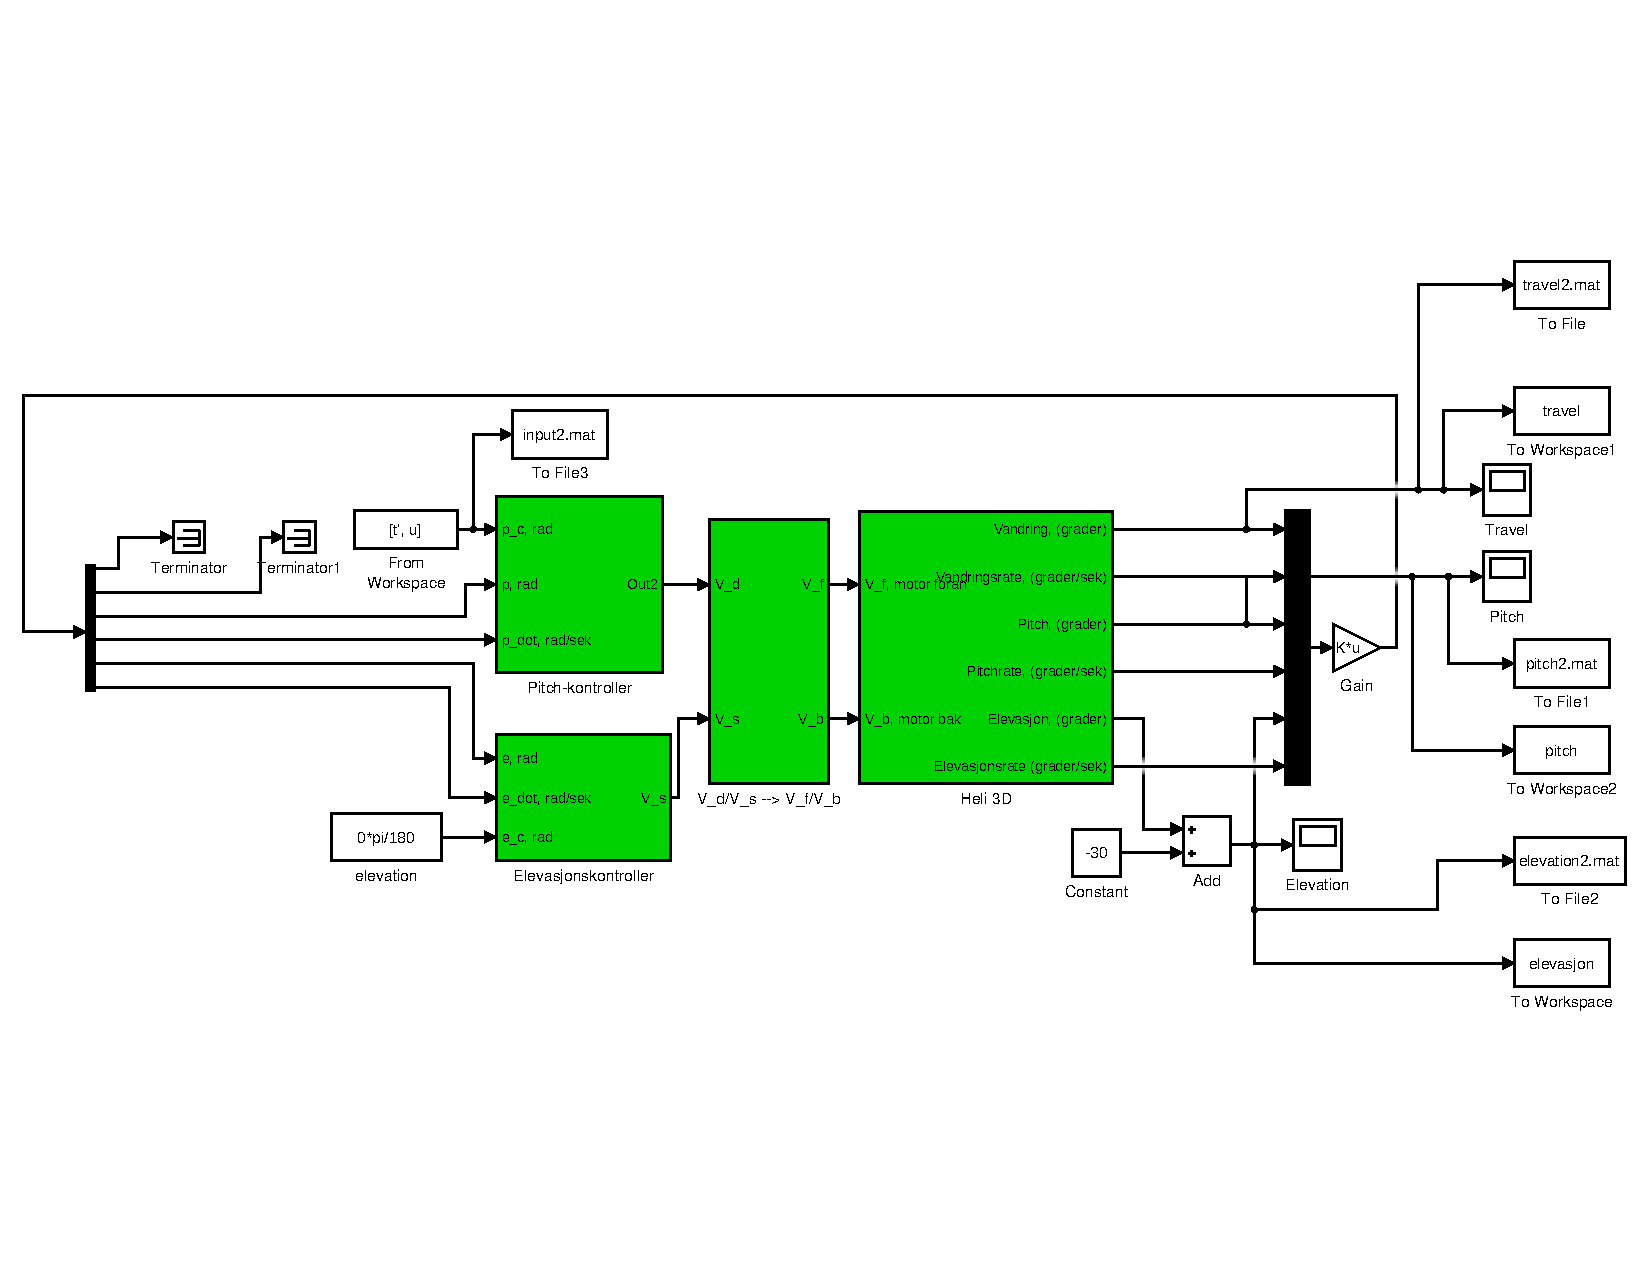
\includegraphics[trim=0 120 0 120,clip,width = \textwidth]{figures/problem2_simulink.pdf}
	\caption{Simulink diagram of problem 2.}
	\label{fig:problem2_simulink}
\end{figure}
\clearpage
\subsection{Problem 3}
\begin{figure}[h]
	\centering
	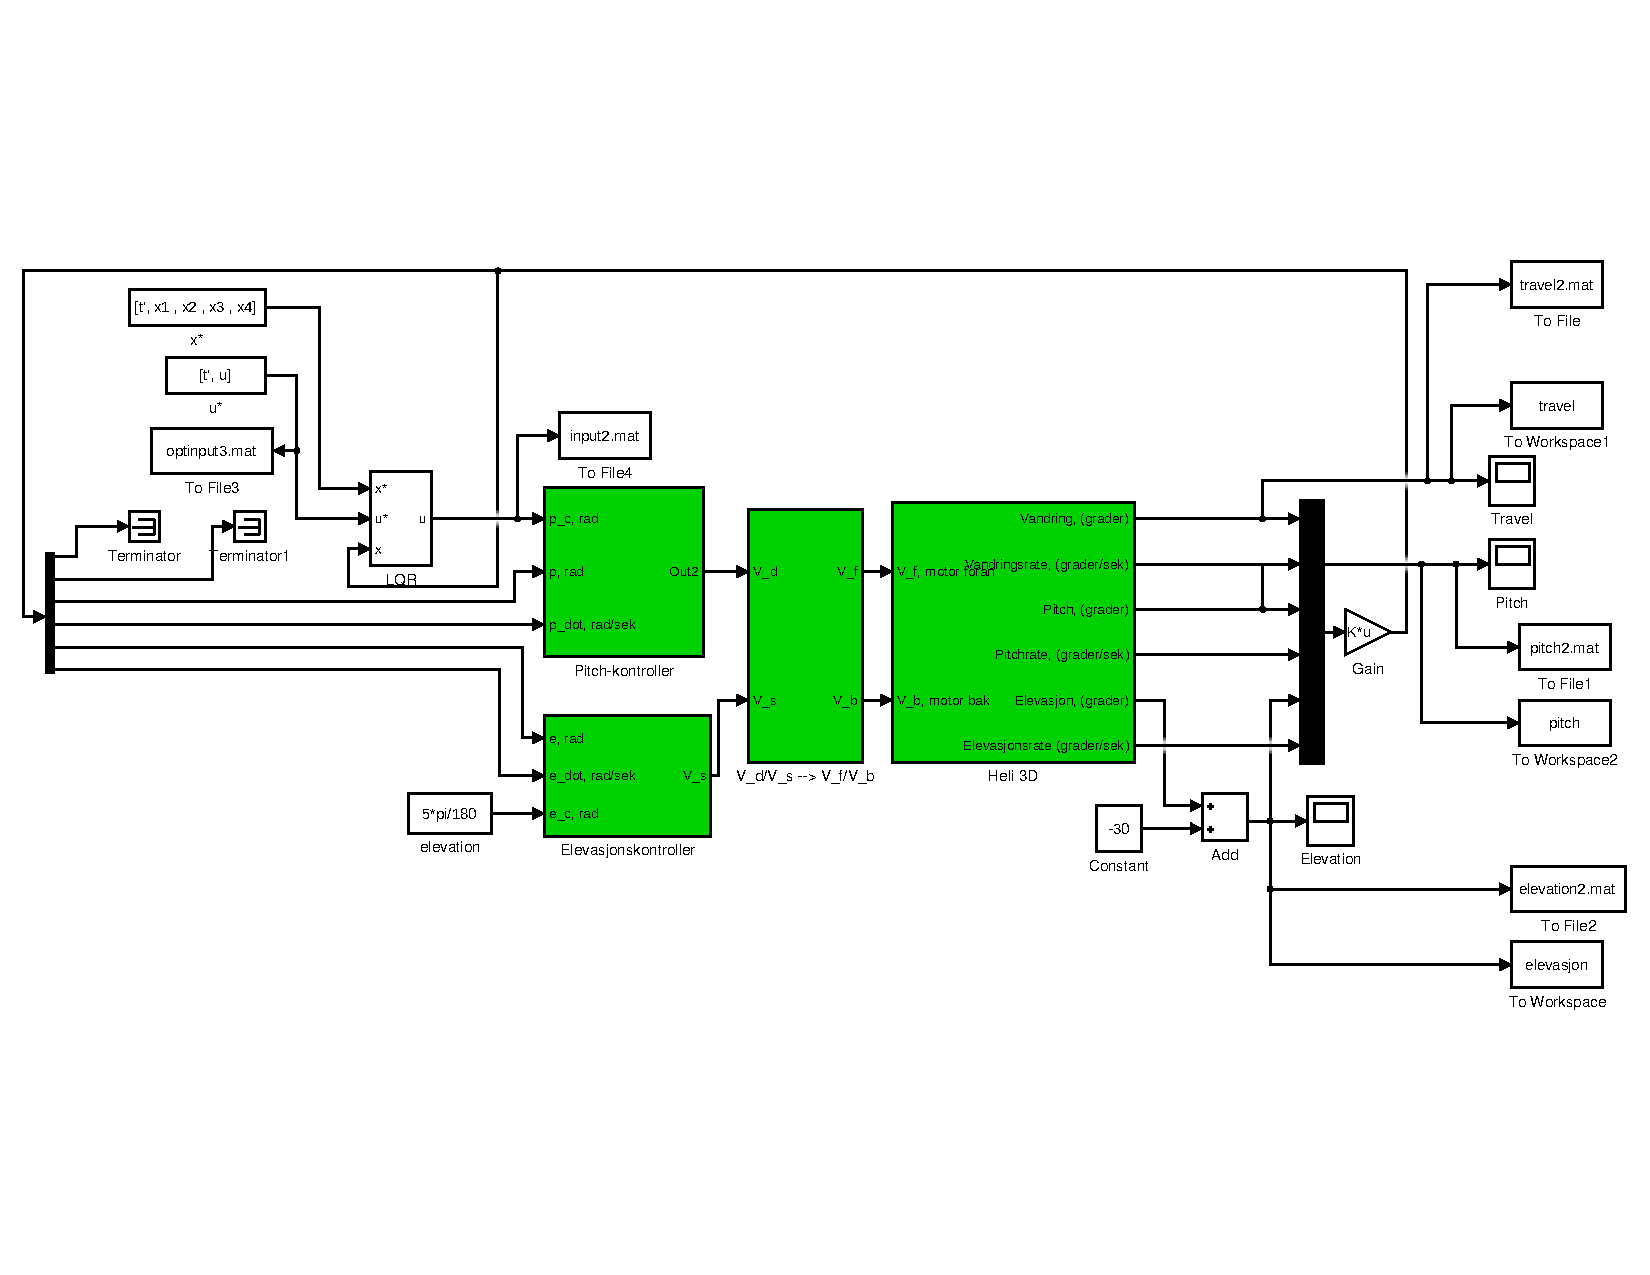
\includegraphics[trim=0 120 0 120,clip,width = \textwidth]{figures/problem3_simulink.pdf}
	\caption{Simulink diagram of problem 3.}
	\label{fig:problem3_simulink}
\end{figure}

\begin{figure}[h]
	\centering
	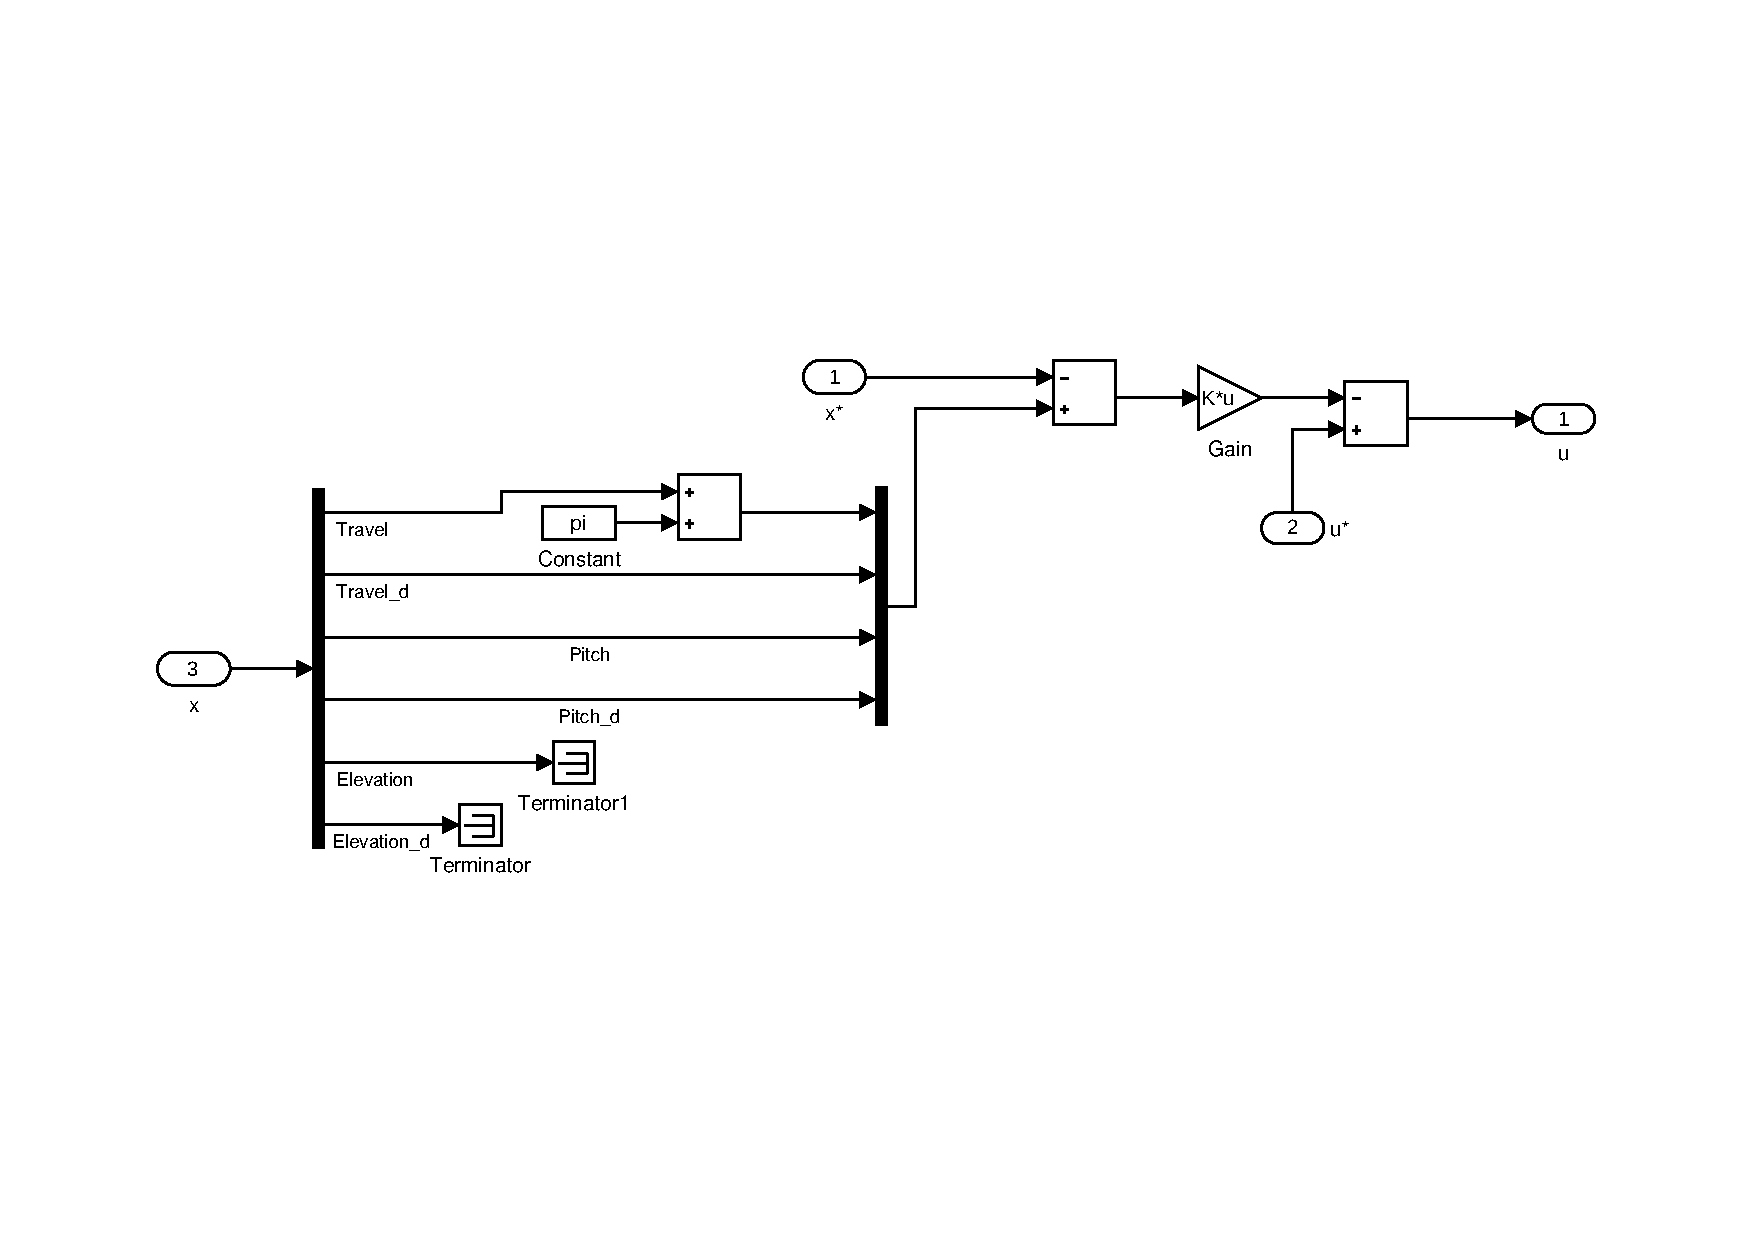
\includegraphics[trim=0 150 0 150,clip,width = \textwidth]{figures/problem3_lqr_simulink.pdf}
	\caption{Simulink diagram of LQR subsystem of problem 3.}
	\label{fig:problem3_lqr_simulink}
\end{figure}
\clearpage
\subsection{Problem 4}
\begin{figure}[h]
	\centering
	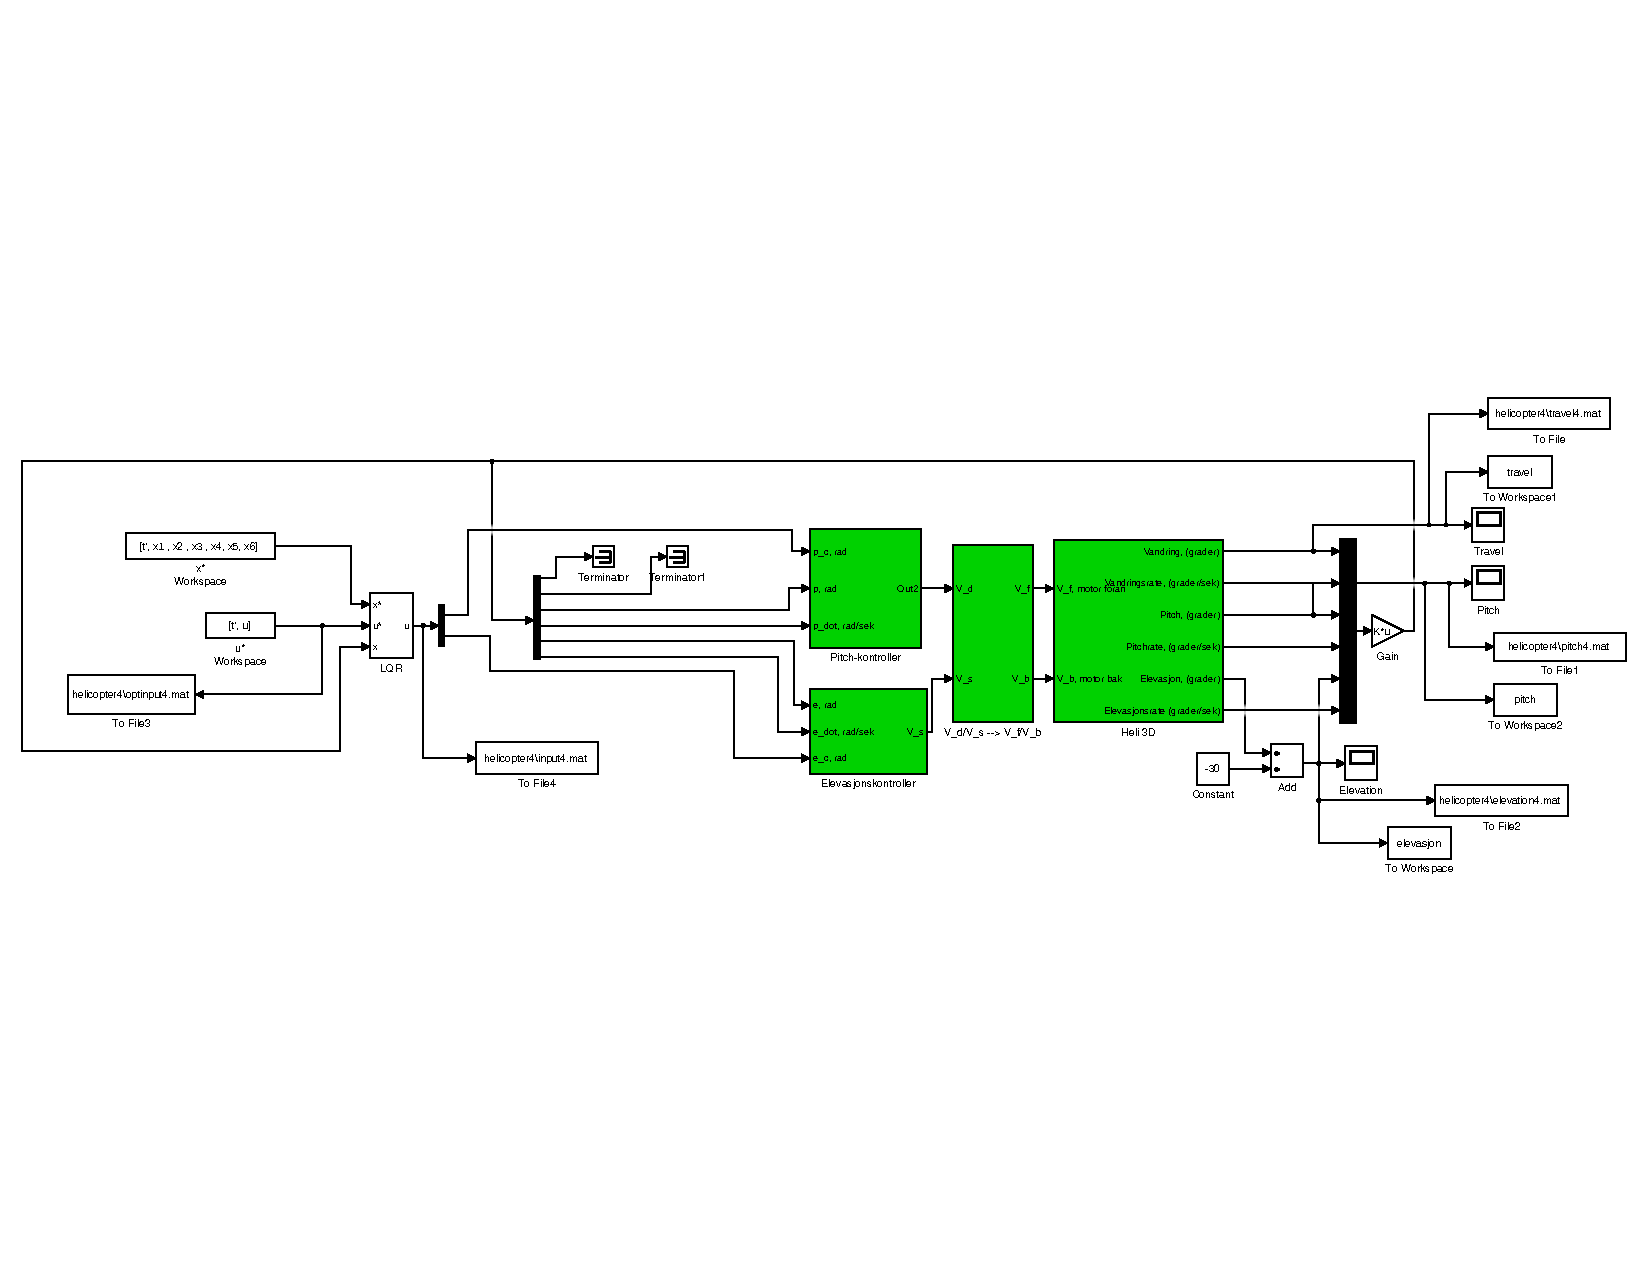
\includegraphics[trim=0 190 0 190,clip,width = \textwidth]{figures/problem4_simulink.pdf}
	\caption{Simulink diagram of problem 4.}
	\label{fig:problem4_simulink}
\end{figure}

\begin{figure}[h]
	\centering
	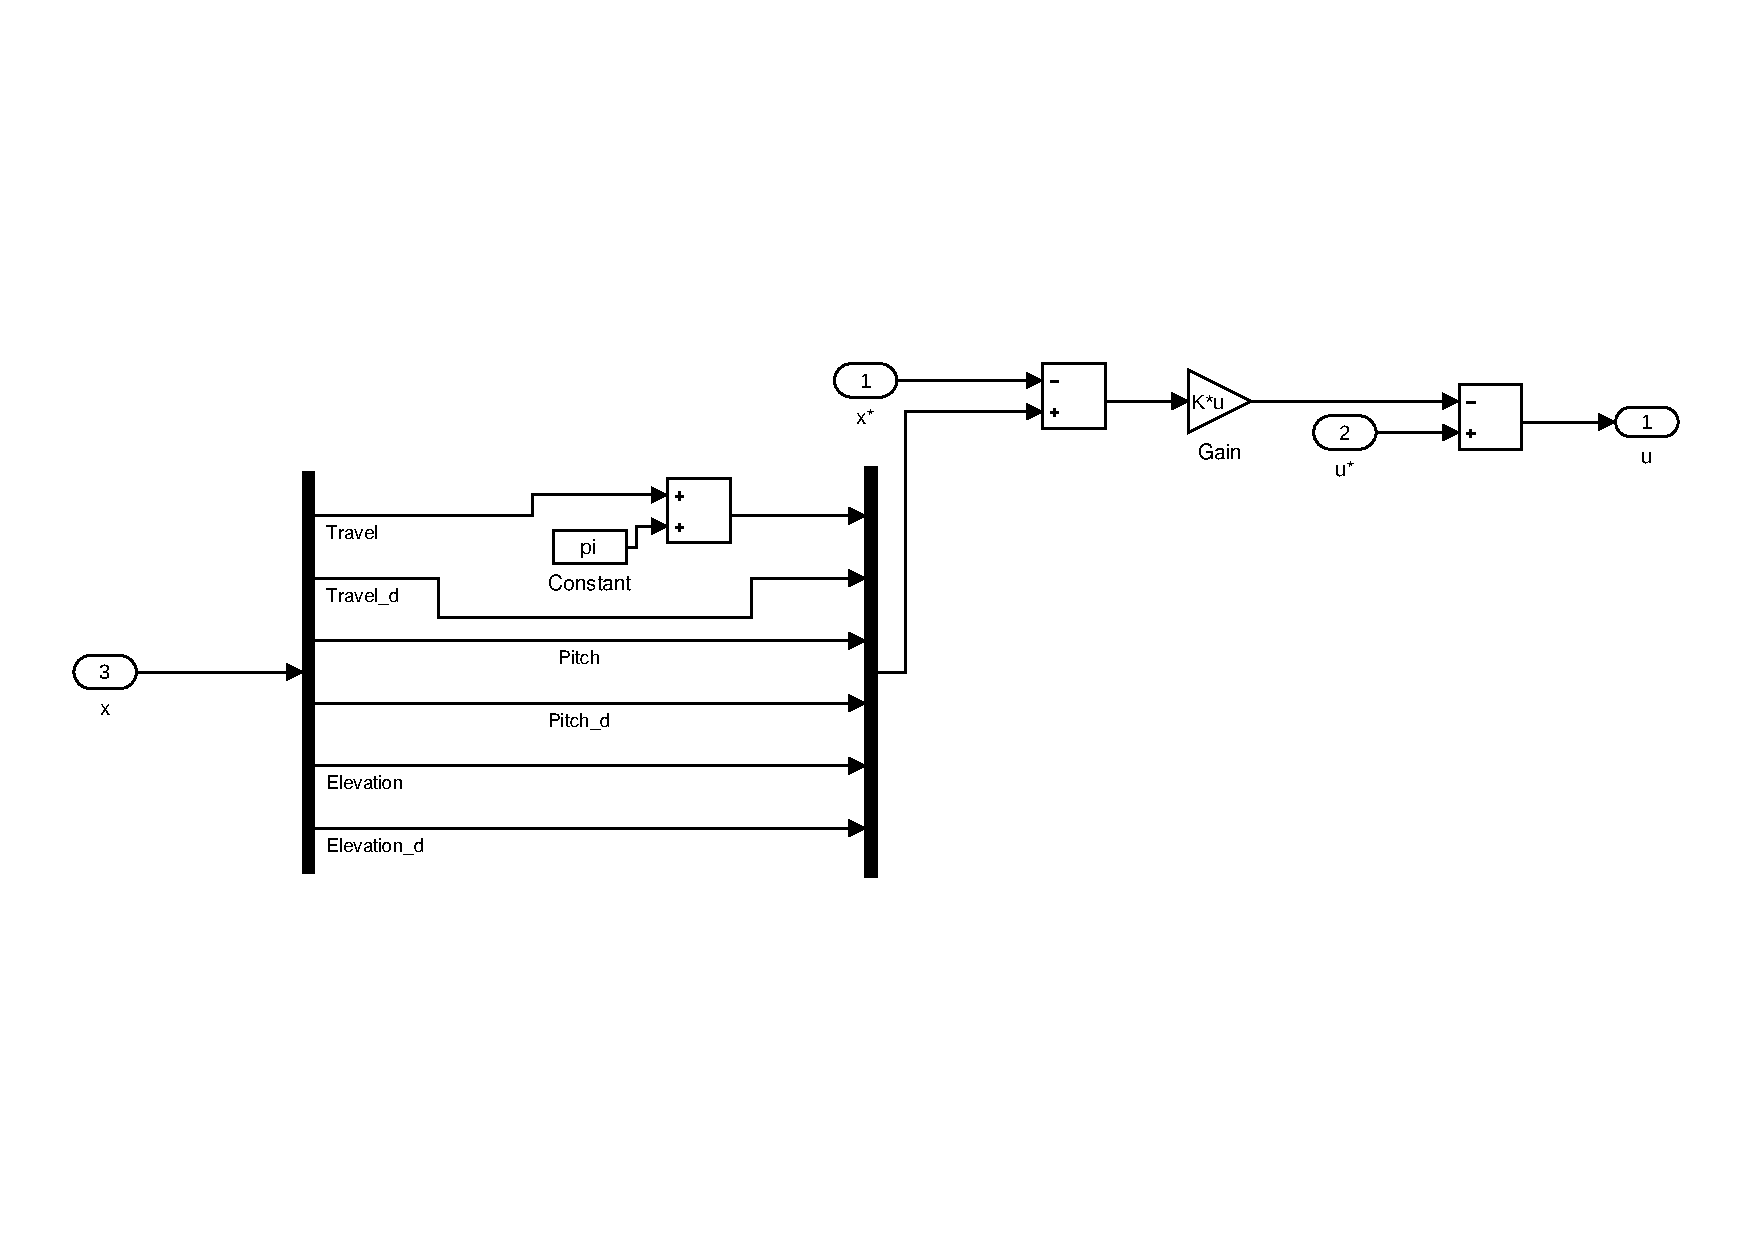
\includegraphics[trim=0 150 0 150,clip,width = \textwidth]{figures/problem4_lqr_simulink.pdf}
	\caption{Simulink diagram of LQR subsystem of problem 4.}
	\label{fig:problem4_lqr_simulink}
\end{figure}


\clearpage
\bibliographystyle{apalike}
\bibliography{helibib}\label{sec:bibliography}


\end{document}
